\documentclass{article}

\usepackage[utf8]{inputenc}
\usepackage[hmargin=2.5cm,vmargin=2.5cm]{geometry}
\usepackage[french]{babel}
\usepackage{amsmath}
\usepackage{graphicx}
\usepackage{stmaryrd}
\usepackage{bbm}
\usepackage{listings}
\usepackage[section]{placeins}
\usepackage{caption}
\usepackage{subcaption}
\usepackage{url}

\usepackage{etoolbox}
\patchcmd{\thebibliography}{\section*}{\section}{}{}

\newcommand{\rapportFigure}{0.45}
\newcommand{\rapportFigureMoyenne}{0.22}
\newcommand{\rapportFigureTierce}{0.13}

\usepackage{color} %red, green, blue, yellow, cyan, magenta, black, white
\definecolor{mygreen}{RGB}{28,140,0} % color values Red, Green, Blue
\definecolor{mylilas}{RGB}{170,55,241}

\lstset{language=Matlab,%
    %basicstyle=\color{red},
    breaklines=true,%
    morekeywords={matlab2tikz},
    keywordstyle=\color{blue},%
    morekeywords=[2]{1}, keywordstyle=[2]{\color{black}},
    identifierstyle=\color{black},%
    stringstyle=\color{mylilas},
    commentstyle=\color{mygreen},%
    showstringspaces=false,%without this there will be a symbol in the places where there is a space
    numbers=left,%
    numberstyle={\tiny \color{black}},% size of the numbers
    numbersep=9pt, % this defines how far the numbers are from the text
    emph=[1]{for,end,break},emphstyle=[1]\color{red}, %some words to emphasise
    %emph=[2]{word1,word2}, emphstyle=[2]{style},    
    frame= single,
}


\usepackage{titlesec} % Used to customize the \section command
\titlespacing{\subsection}{0pt}{10pt}{10pt}
\titlespacing{\subsubsection}{0pt}{10pt}{10pt}
\titlespacing{\section}{0pt}{10pt}{10pt}

\title{Méthodes à haute résolution}
\author{Augustin HOFF et Gustavo CIOTTO PINTON}
\date{2014}

\begin{document}


\begin{titlepage}
\vspace*{.28\textheight}
\begin{center}
%
\begin{figure}[h]
    \centering
    
\includegraphics[scale=0.12]{images/LogoSupelec}
\end{figure}
%
\vspace*{10pt}
%\text{ }\\[7 cm]
\textbf{\LARGE METHODES A HAUTE RESOLUTION}\\[2 cm]
Augustin \textbf{HOFF} et Gustavo \textbf{CIOTTO PINTON}\\[1 cm]
Projet de synthèse, Supélec, 2014

\end{center}
\end{titlepage}

\newpage
\tableofcontents

\newpage

\section{Généralités}

\subsection{Introduction}

Le but de ce projet est d'étudier les méthodes à haute résolution à travers la compréhension et l'approfondissement d'algorithmes connus sur ce sujet comme MUSIC. L'implémentation de ce dernier sur Matlab va permettre de mettre en pratique les études théoriques abstraites basées sur des statistiques ou des espaces hermitiens par exemple.


Une méthode à haute résolution est une méthode qui permet de mesurer des directions (ou des positions ou des fréquences en analyse spectrale) avec une erreur qui n‘est limitée, dans le cas idéal, que par la durée d'observation du phénomène. Elle permet donc de résoudre le problème suivant: comment peut-on décrire la distribution géographique et
même fréquentielle de sources finies à partir seulement de données fournies par des capteurs
(le bruit constituera ici la principale difficulté).


Des applications sont toutes trouvées comme le sonar ou encore le radar, où le principe consiste à déterminer la direction d'arrivée des ondes électromagnétiques (radar) ou 
acoustiques (sonar) afin de localiser les sources. 


Les signaux étudiés seront aléatoires à composante exponentielle (complexe) et feront intervenir des notions de probabilité.


\vspace*{20pt}

% http://hal.archives-ouvertes.fr/docs/00/44/74/88/PDF/These_Carine_EK.pdf


\subsection{Outils mathématiques } 


\subsubsection{Quelques définitions}

\begin{itemize}\renewcommand{\labelitemi}{$\bullet$}

\item L'autocorrelation d'un processus aléatoire pour deux indices de temps différents \(n_1\) et \(n_2\) est définie comme

\begin{equation}
%
    \label{eq:autocorr} 
    r_{xx} = \mathcal E \{ x[n_1]x^*[n_2] \}
%
\end{equation}

\vspace*{15pt}

\item L'autocovariance est définie comme

\begin{equation}
%
    \label{eq:autocov} 
    c_{xx}[n_1,n_2] = \mathcal E \{(x[n_1]-\overline{x}[n_1])(x^*[n_2]-\overline{x}^*[n_2])\}
%
\end{equation}

où 

\begin{equation}
    \label{eq:mean} 
    \overline{x}[n] = \mathcal E \{x[n]\}
\end{equation}

D'après les équations \ref{eq:autocorr} et \ref{eq:autocov}, on peut alors écrire 

\begin{equation}
%
    \label{eq:autocovcorr} 
    c_{xx}[n_1,n_2] = r_{xx}-\overline{x}[n_1]\overline{x}^*[n_2]
%
\end{equation}

On note ainsi que si la moyenne est nulle, l'autocovariance est égale à l'autocorrelation.
\vspace*{20pt}

\item Un processus aléatoire est dit stationnaire au sens large (\textit{wide-sense stationary} en anglais) si \(\overline{x}[n] = \mathcal E\{x[n]\} = constante\) \( \forall n\), et si son autocorrelation dépend seulement de la différence  \(m = n_2 - n_1 \). En résumé

\[\overline{x}[n] = \overline{x}\] et
\begin{equation}
        \label{eq:autocorrwss} 
    r_{xx}[m] = \mathcal E \{ x[n + m]x^*[n] \}
\end{equation}

\vspace*{15pt}

\item Quelques propriétés remarquables peuvent être listées comme, par exemple

\[r_{xx}[0] \ge |r_{xx}[m]|\] 

et 

\[r_{xx}[-m] = r_{xx}^*[m]\]

\vspace*{15pt}

\item La matrice formée par les valeurs d'autocorrelation est notée \(R_{N-1}\) et est écrite comme

\begin{equation}
%
    \label{eq:matricecorr}
    R_{N-1}=\begin{bmatrix}
        r_{xx}[0] & r_{xx}[-1] & r_{xx}[-2] & \cdots & r_{xx}[-(N-1)] \\
        r_{xx}[1] & r_{xx}[0] & r_{xx}[-1] & \cdots & r_{xx}[-(N-2)] \\
        \vdots & \vdots & \vdots & \ddots & \vdots \\
        r_{xx}[N-1] & r_{xx}[N-2] & r_{xx}[N-3] & \cdots & r_{xx}[0] \\
    \end{bmatrix}
%
\end{equation}

\vspace*{15pt}

\item Le rapport entre les puissances du signal et du bruit est appellé SNR (\textit{Signal-to-Noise Ratio}) dont expression est donnée par 

\begin{equation}
    SNR = \frac{P_{signal}}{P_{bruit}}
\end{equation}

Il est souvent écrit en \textit{décibels} [dB]:

\begin{equation}
    \label{eq:snr}
    SNR_{dB} = 10* \log \left[ \frac{P_{signal}}{P_{bruit}} \right]
\end{equation}

\item La puissance d'un processus aléatoire est calculée par l'équation suivante

\begin{equation}
    P_x = \frac{1}{2\pi} \int_{-\pi}^{\pi}  S_x (\omega) d\omega = \int_{-\frac{1}{2}}^{\frac{1}{2}}  S_x (\nu) d\nu
\end{equation}

où \(S_x(f) = \mathcal{F} \{r_{xx}[k]\}\), la transformée de Fourier de la fonction d'autocorrelation, est appellé la \textit{densité spectrale de puissance}. Pour les processus stationnaires, on note que

\begin{equation}
    \label{eq:puissance}
    P_x = r_{xx} [0]
\end{equation}

\underline{Démonstration}:

\[ P_x = \frac{1}{2\pi} \int_{-\pi}^{\pi}  S_x (\omega) d\omega = \frac{1}{2\pi} \int_{-\pi}^{\pi} \left( \sum_{k = - \infty}^{\infty} r_{xx}[k] \exp(-j \omega k) \right) d\omega  = \]  
\[ = \sum_{k = - \infty}^{\infty} r_{xx}[k]  \left( \int_{-\pi}^{\pi}  \exp(-j \omega k) d\omega \right) = \sum_{k = - \infty}^{\infty} r_{xx}[k] \delta [k] = r_{xx} [0] \]

\end{itemize}

%http://www.idsc.ethz.ch/Courses/signals_and_systems/ArchiveFall10/lectureNotes8.pdf

\newpage

\subsubsection{Application à un signal sinusoïdal complexe}

Dans notre cas, on considère \(s[n]\) comme une somme de P sinusoïdes complexes telles que 

\begin{equation}
\label{eq:x}
    s[n] = \sum_{k=1}^{P} A_k \exp(j(2\pi f_k n T + \theta _k))
\end{equation}

T correspond à la période d'échantillonnage.
On suppose que les variables aléatoires \(\theta _k\) sont idépendantes et uniformement distribuées sur l'intervalle \( [0, 2\pi[\). Ainsi le calcul de la moyenne et de l'autorrelation pour s[n] est simplifié et donne grâce à \ref{eq:autocorr} et \ref{eq:mean} : 

\begin{equation}
\label{eq:meanx}
    \overline{s}[n] = 0
\end{equation}

et

\begin{equation}
\label{eq:rxx}
    r_{ss}[m] = \sum_{k=1}^{P} A_k^2 \exp(j 2\pi f_k m T)
\end{equation}

\vspace*{10pt}

\underline{Démonstration}:

%\begin{align*}
\[ \overline{s}[n] = \int_{-\infty}^{\infty} A_k \exp(j (2\pi f_k n T + \theta)) \frac{\mathbf{1}_{[0, 2\pi[}}{2\pi}\, \mathrm{d}\theta = 0  \]

et 

\[ r_{xx}[n_1,n_2] = \mathcal E \{ s[n_1]s^*[n_2] \} = \mathcal E \{ \sum_{i=1}^{P} A_i \exp(j(2\pi f_i (n_1) T + \theta _i))(\sum_{j=1}^{P} A_j^* \exp(-j(2\pi f_j n_2 T + \theta _j)) \} = \] 

\[  =  \mathcal E \{ \sum_{i=1}^{P} A_i^2 \exp(j 2\pi f_i (n_1-n_2) T)\} + \mathcal E \{ \sum\limits_{\substack{(i,j) \in \llbracket 1,P\rrbracket  \\ i \neq j}}  A_i A_j^* \exp(j(2\pi ( f_i n_1 - f_j n_2) T + \theta _i - \theta_j)) \}  \]
%\end{align*}


En effet, les \( \theta_k \) étant indépendantes, alors les variables aléatoires résultantes d'une composition avec une exponentielle le sont aussi (car c'est une fonction continue donc mesurable). On en déduit que

%\vspace*{20pt}

\[ \mathcal E \{ \sum\limits_{\substack{(i,j) \in \llbracket 1,P\rrbracket  \\ i \neq j}}  A_i A_j^* \exp(j(2\pi ( f_i n_1 - f_j n_2) T + \theta _i - \theta_j)) \} = \]
\[=  \sum\limits_{\substack{(i,j) \in \llbracket 1,P\rrbracket  \\ i \neq j}} \mathcal E \{ A_i \exp(j(2\pi f_i n_1 T + \theta _i)) \} \mathcal E \{ A_j^* \exp(-j(2\pi f_j n_2 T + \theta _j)) \} \]

%\vspace*{20pt}

Ce terme est donc nul de la même façon que pour le calcul de \( \overline{s}[n]\).
Le terme restant donne le résultat.

On note que le processus \(s[n]\) est stationnaire (WSS). 




\newpage

Par analogie avec la lumière blanche qui contient toutes les fréquences lumineuses avec la même intensité, un bruit blanc est un processus stochastique qui possède la même densité spectrale de puissance à toutes les fréquences. Ceci correspond à une autocorrélation nulle en tout point sauf à l'origine : le processus est décorrélé.

\vspace*{15pt}

Si on ajoute alors un bruit blanc \(w[n]\) de variance \(p_w\) à \(s[n]\), le processus \(x[n] = s[n] + w[n]\) aura comme autocorrelation l'expression

\begin{equation}
\label{eq:ryy}
    r_{xx}[m] = r_{ss}[m] + r_{w}[m] = \sum_{k=1}^{P} A_k^2 \exp(2\pi f_k m T) + p_w\delta [m]
\end{equation}

et matrice d'autocorrelation 

\begin{equation}
%
    \label{eq:Ryy}
    R_{xx}= R_{ss} + R_w =\sum_{k=1}^{P}A_k^2 \boldsymbol{e}_{N-1}(f_k) \boldsymbol{e}_{N-1}^H(f_k) + p_w\boldsymbol{I}
%
\end{equation}

où 

\begin{equation}
%
    \label{eq:em}
    \boldsymbol{e}_{N-1}(f_k)=\begin{bmatrix}
        1 \\
        \exp (2 \pi j f_k T) \\
        \vdots \\
        \exp (2 \pi j f_k (N-1)T) \\
    \end{bmatrix}
%
\end{equation}

\vspace*{15pt}

Les deux matrices \(R_{ss}\) et \(R_{w}\) ont pour dimension \(N\times N\).

\vspace*{15pt}

Enfin, on calcule la puissance associée au signal d'entrée à partir de l'équation \ref{eq:puissance}. Cela donne

\begin{equation}
    P_{ss} = r_{ss} [0] = \sum_{k=1}^{P}A_k^2
\end{equation}

et d'après l'équation \ref{eq:snr}, on obtient le rapport signal-bruit (SNR) correpondant

\begin{equation}
    SNR_{dB} = 10* \log \left[ \frac{P_{signal}}{P_{bruit}} \right] = 10* \log \left[ \frac{\sum_{k=1}^{P}A_k^2}{p_w} \right]
\end{equation}


\newpage
%-----------------------------------------


\subsubsection{Estimation de fréquences par l'analyse des éléments propres}

Étant donnée l'équation \ref{eq:Ryy}, on peut en déduire que si la matrice d'autocorrelation a un ordre \(N\) plus grand ou égal au nombre de sinusoïdes complexes \(P\), i.e \(N - 1 > P\), alors la matrice d'autocorrelation des signaux, \(R_{ss}\) a pour rang \(P\). 
En effet, les vecteurs \( \boldsymbol{e}_{N-1}(f_k) \) engendrent l'image de \(R_{ss}\).
Cela peut se voir soit en revenant à la définition \ref{eq:matricecorr}, soit en remarquant tout simplement que \( \boldsymbol{e}_{N-1}(f_k) \boldsymbol{e}_{N-1}^H(f_k)\) est un des \(P\) projecteurs de rang 1.

\vspace*{10pt}

De façon plus simple , on peut vérifier que la matrice d'autocovariance du bruit \(R_w\) a rang \(N\) puisqu'elle est multiple d'une matrice identité \(N\times N\).

\vspace*{20pt}

En outre, la matrice \(R_{ss}\) qui est hermitienne par définition peut être écrite grâce à ses valeurs et vecteurs propres

\begin{equation}
\label{eq:eigen}
R_{ss}=\sum_{i=1}^{N}\lambda _i \boldsymbol{v}_{i} \boldsymbol{v}_{i}^H
\end{equation}

où \(\lambda _1 > \lambda _2 > \lambda _3 > \hdots > \lambda _N  \geq 0\) et \(\boldsymbol{v}_{i} \boldsymbol{v}_{j}^H = 0\) si \(i \neq j\) et 1 sinon (vecteurs orthogonaux et de norme 1). 

\vspace*{20pt}

On peut démontrer\footnote{ Le théorème du rang donne la dimension du noyau: N-P} qu'une matrice de dimension \(N\) avec \(P < N\) a \(N - P\) valeurs propres égales à 0. L'équation \ref{eq:eigen} devient donc 

\begin{equation}
\label{eq:eigenM}
R_{ss}=\sum_{i=1}^{P}\lambda _i \boldsymbol{v}_{i} \boldsymbol{v}_{i}^H
\end{equation}

Une representation alternative de la matrice identité \(N \times N\) en fonction des vecteurs propres est

\begin{equation}
\label{eq:identite}
\boldsymbol{I}=\sum_{i=1}^{N} \boldsymbol{v}_{i} \boldsymbol{v}_{i}^H
\end{equation}
 
En remplaçant les équations \ref{eq:eigenM} et \ref{eq:identite} dans \ref{eq:Ryy} on obtient

\begin{equation}
%
    \label{eq:RyyEigen}
    R_{xx}= R_{ss} + R_w =\sum_{i=1}^{P}\lambda _i \boldsymbol{v}_{i} \boldsymbol{v}_{i}^H + p_w\sum_{i=1}^{N} \boldsymbol{v}_{i} \boldsymbol{v}_{i}^H = \sum_{i=1}^{P}(\lambda _i + p_w) \boldsymbol{v}_{i} \boldsymbol{v}_{i}^H + p_w\sum_{i=P+1}^{N} \boldsymbol{v}_{i} \boldsymbol{v}_{i}^H
%
\end{equation} 

Ainsi, les vecteurs propres \(\boldsymbol{v}_{P+1}, \boldsymbol{v}_{P+2}, \hdots, \boldsymbol{v}_{N} \) construisent l'espace bruit de \(R_w\), tous avec la même valeur propre \(p_w\) et les vecteurs \(\boldsymbol{v}_{1}, \boldsymbol{v}_{2}, \hdots, \boldsymbol{v}_{P} \), dits principaux, construisent l'espace des signaux de \(R_{xx}\) et \(R_{ss}\) avec comme valeurs propres \(\lambda _1 + p_w, \lambda _2 + p_w, \hdots, \lambda _P + p_w\). 

\vspace*{10pt}

C'est important de remarquer que les valeurs propres des vecteurs principaux dépendent du signal mais aussi du bruit, ce qui peut générer des complications dans le cas où la variance du bruit blanc est relativement grande.

\vspace*{10pt}

Enfin, des algorithmes (comme \textit{MUSIC} et \textit{ESPRIT}), abordés plus précisement dans la suite, sont basés sur le fait que les vecteurs qui répresentent les signaux sont tous orthogonaux aux vecteurs qui décrivent le bruit. Ainsi, lorsqu'une entrée \(\boldsymbol{s}\) est captée, il est possible déterminer si une telle entrée est essentiellement composée de bruit ou non grâce au produit scalaire

\begin{equation}
    \label{eq:produit}
    \boldsymbol{s}^H \left( \sum_{k=P+1}^{N} \alpha _k  \boldsymbol{v}_k \right)
\end{equation}
qui théoriquement vaut 0 si l'entrée est un signal sinusoïdal complexe.

\newpage














\section{Algorithme MUSIC}

\subsection{Aspect théorique}

L'algorithme MUSIC\footnote{MUltiple SIgnal Classification} se base exactement sur le même principe que l'équation \ref{eq:produit} pour détecter des pics mais, par contre, utilise une autre expression qui dépend explicitement de la fréquence. Celle-ci s'écrit:

\begin{equation}
%
    \label{eq:basemusic}
    \sum_{k=P+1}^{N} \alpha _k \left| \boldsymbol{e}_{N-1}^H (f) \boldsymbol{v}_k \right| ^2 = \boldsymbol{e}_{N-1}^H (f) \left( \sum_{k=P+1}^{N} \alpha _k  \boldsymbol{v}_{k}\boldsymbol{v}_k^H \right) \boldsymbol{e}_{N-1} (f)
%
\end{equation}
%
où, seulement pour cet algorithme, \( \alpha _k = 1 \) \(\forall k\). 

\vspace*{10pt}

On a que \ref{eq:produit}, \ref{eq:basemusic} valent 0 si \(\boldsymbol{e}_{N-1}(f)\) est un des vecteurs de l'espace signal i.e si \( f = f_k \) pour k \( \in \llbracket 1,P\rrbracket \), puisqu'il est orthogonal à toute combinaison linéaire des vecteurs qui construisent l'espace du bruit.

L'estimateur est donc donné par l'expression

\begin{equation}
%
    \label{eq:music}
    P_{MUSIC} (f) = \frac{1}{\boldsymbol{e}_{N-1}^H (f) \left( \sum_{k=P+1}^{N}   \boldsymbol{v}_{k}\boldsymbol{v}_k^H \right) \boldsymbol{e}_{N-1} (f)}
%
\end{equation}
  et tend vers l'infini pour des fréquences qui composent le signal.

\vspace*{10pt}

\subsection{Mise en oeuvre}
\label{miseenouvre}

\vspace*{10pt}

En s'appuyant sur la théorie, on peut alors écrire un algorithme afin de déterminer les fréquences d'un signal source dissimulé dans du bruit. Le resultat est obtenu grâce à la détermination des pics de la fonction Pmusic, explicitée ci-dessus. 
Voici le code détaillé :

\vspace*{20pt}

\lstinputlisting[language=Matlab]{source/P_music.m}

\newpage

Après avoir écrit l'algorithme principal, on réalise une fonction test avec les mêmes notations que pour la théorie.

\vspace*{20pt}

\lstinputlisting[language=Matlab]{source/test.m}

\subsection{Resultats}

Les figures representées ci-dessous sont les résultats des programmes présentés dans la section \ref{miseenouvre} pour différentes valeurs du SNR (eq. \ref{eq:snr}) à un  nombre de mesures constant \(N = 100\). Afin de mieux mettre en évidence l'évolution des pics, nous avons adopté \(P = 3\) dans nos tests, contrairement à \( P = 2\) indiqué par le sujet. Les fréquences du signal d'entrée choisies, et qui alors doivent être identifiés par le programme, sont  \(f_1 = 49Hz\), \(f_2 = 50Hz\) et \(f_3 = 60Hz\).  Les deux premières ont été choisis très proches, ce qui peut, dans les cas où la puissance du signal n'est pas assez forte comparée à celle du bruit, compliquer leur identification. Enfin, les amplitudes utilisées sont \(A_1 = 1\), \(A_2 = 2.5\) et \(A_3 = 3\).

\vspace*{10pt}

Dans chacune des figures, on trouve deux graphiques: le premier, au dessus, répresente le résultat de l'éxécution de la fonction P\textsuperscript{music} pour fréquences comprises dans l'interval de \(1 Hz\) jusqu'à \(100Hz\), et le deuxiéme montre la transformée de Fourier discrète du respectif signal x, \(X( \nu ) = \mathcal{F} \{x[k]\}\) ,  réalisée à partir de la commande \textit{fft}, implementée sous Matlab. L'objectif de cette approche consiste à comparer les méthodes conventionnelles d'analyse fréquentielle à celles dites de haute résolution, afin de déterminer les situations où la \textit{fft} n'arrive pas à identifier des fréquences proches. 

\vspace*{10pt}

La figure \ref{fig:snr0001} répresente la sortie du programme pour \(SNR = 0.001dB\), situation où les puissances sont presque égales ( \( \frac{P_s}{P_b} = 10^{\frac{0.001}{10}} \approx 1 \) ) et, par conséquent, dans ce cas là, le bruit interfère fortement dans le signal \(x(t)\), comme l'illustre la figure \ref{fig:wave0001}. On vérifie déjà que la fréquence correpondante à \( f_1 = 49Hz\) est indiscernable aux deux méthodes et que les pics obtenus par la fonction P\textsuperscript{music} ne sont pas aussi accentués comme ceux des figures \ref{fig:snr100} et \ref{fig:snr500}, dont les ordres de grandeur sont de \(10^{10}\) et \(10^{14}\) respectivement. On vérifie aussi que le bruit intense a provoqué l'apparition de certains sommets pour fréquences qui n'appartiennent pas au signal original dans les deux figures.

%
\begin{figure}[h]
    \centering
    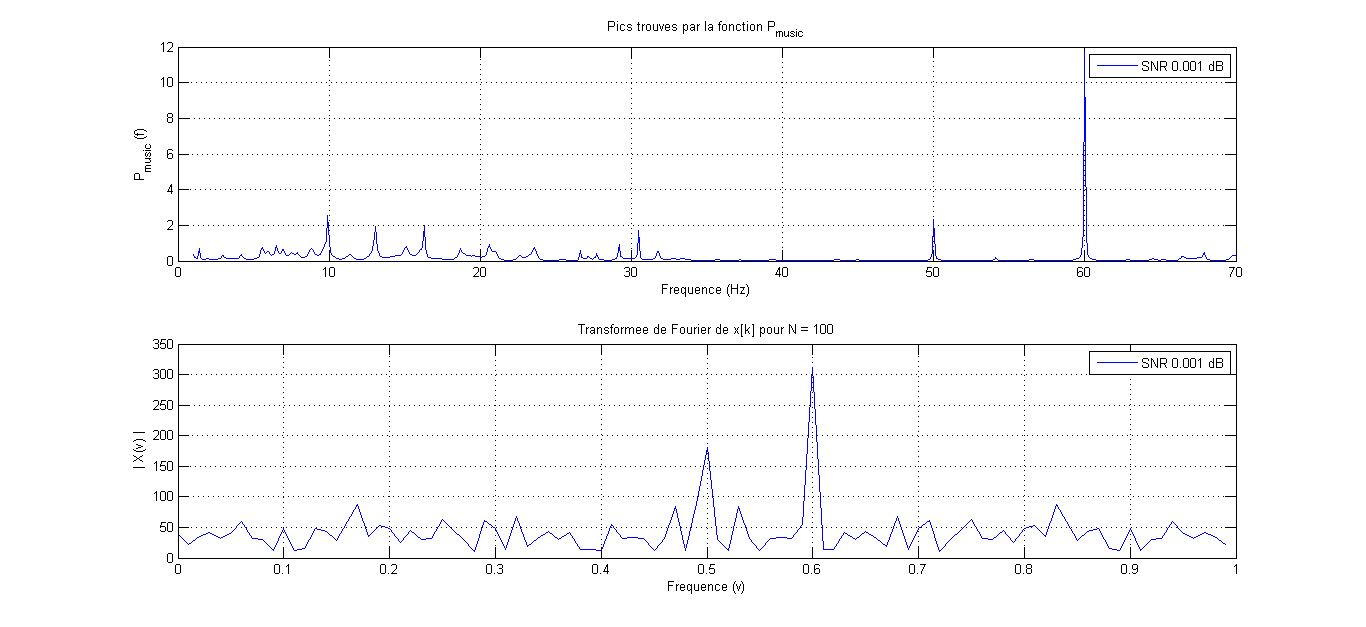
\includegraphics[scale= \rapportFigure]{images/snr0001}
    \caption{Resultats obtenus pour \(SNR_{dB} = 0.001 dB\)}
    \label{fig:wave0001}
\end{figure}
%


%
\begin{figure}[h]
    \centering
    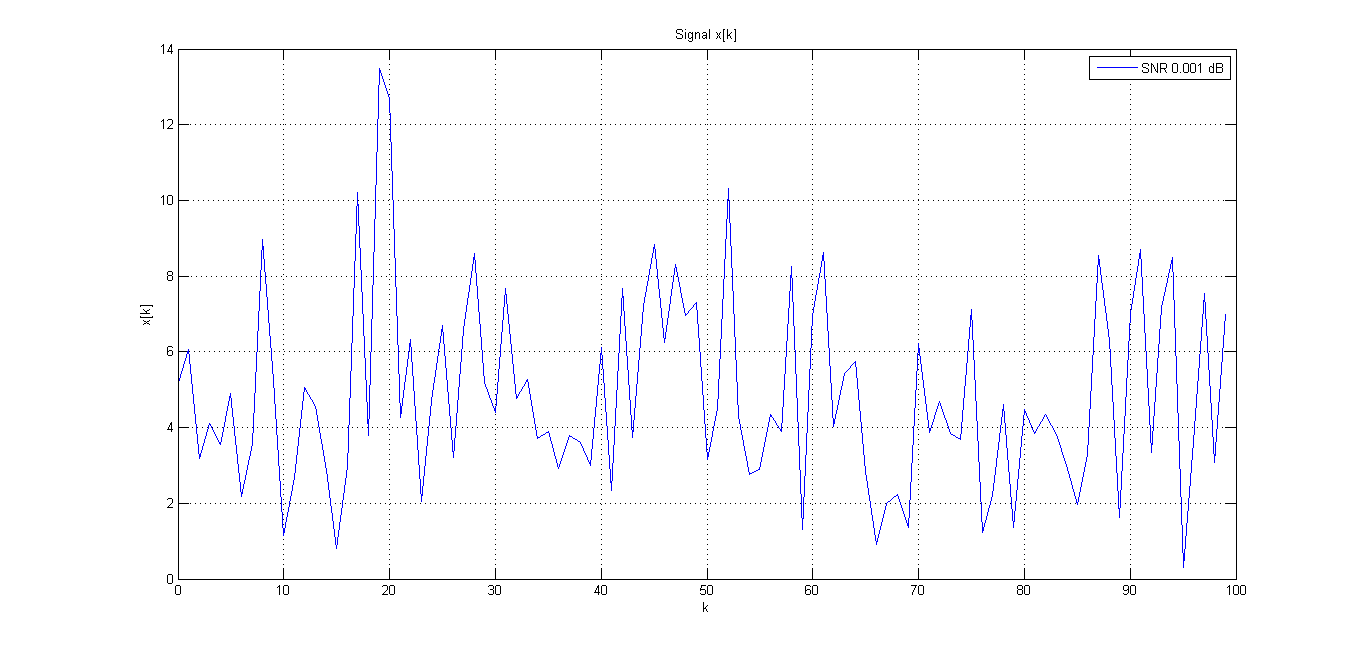
\includegraphics[scale= \rapportFigure ]{images/wave0001}
    \caption{Signal avec du bruit pour \(SNR_{dB} = 0.001 dB\)}
    \label{fig:snr0001}
\end{figure}
%


\FloatBarrier

Les figures \ref{fig:snr40} et \ref{fig:snr100} montrent les résultats de l'éxécution pour \(SNR = 40dB\) et \(SNR = 100dB\), c'est-à-dire que la puissance du  signal est assez grande comparée à celle du bruit. Plus spécifiquement, \(P_s = 10^{\frac{40}{10}}P_b\) et \(P_s = 10^{\frac{100}{10}}P_b\) respectivement. Dans ces deux cas, on vérifie que les pics correspondants aux fréquences ajoutées par le bruit disparaissent, restant seulement ceux du signal. Par contre, l'algorithme \textit{MUSIC} est déjà capable d'identifier séparément \(f_1 = 49Hz\) et \(f_2=50Hz\) (le pic relatif à \(f_1\) est faible comparé aux autres mais  peut être bien distingué quand même). Néanmoins la transformée de Fourier n'a pas été capable quand à elle de distinguer ces deux fréquences.

\vspace*{10pt}

On comprend donc l'intérêt ici des méthodes hautes résolution: les pics sont beaucoup plus accentués et localisés que ceux générés par la transformée.

%mais, par contre, toutes les fréquences ne sont pas encore identifiables. Cela n'apporte pas donc grand chose %de plus par rapport au premier cas puisque les pics même avec une "petite" amplitude étaient déjà bien visibles.

\FloatBarrier


\begin{figure}[h]
%
    \centering
    \begin{subfigure}{0.49\textwidth}
        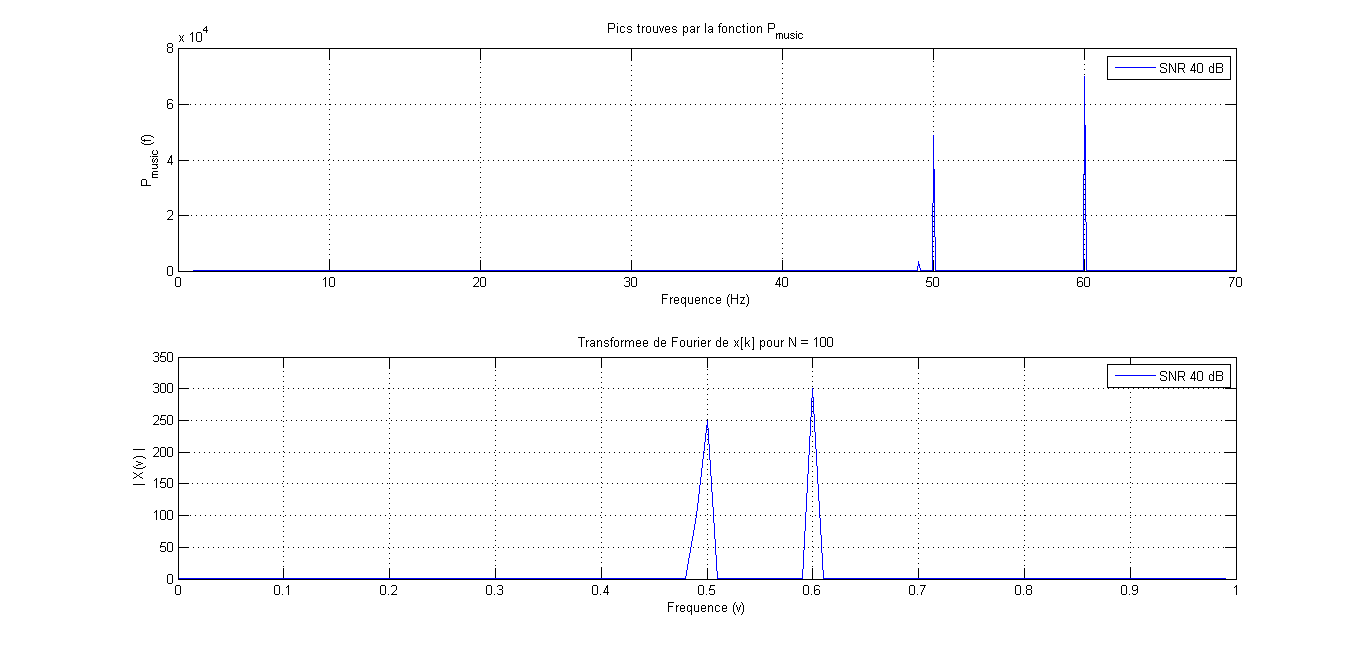
\includegraphics[scale=\rapportFigureMoyenne ]{images/snr40}
        \caption{\(SNR_{dB} = 40 dB\)}
        \label{fig:snr40}
    \end{subfigure}
    %
    ~
    %
    \begin{subfigure}{0.49\textwidth}
        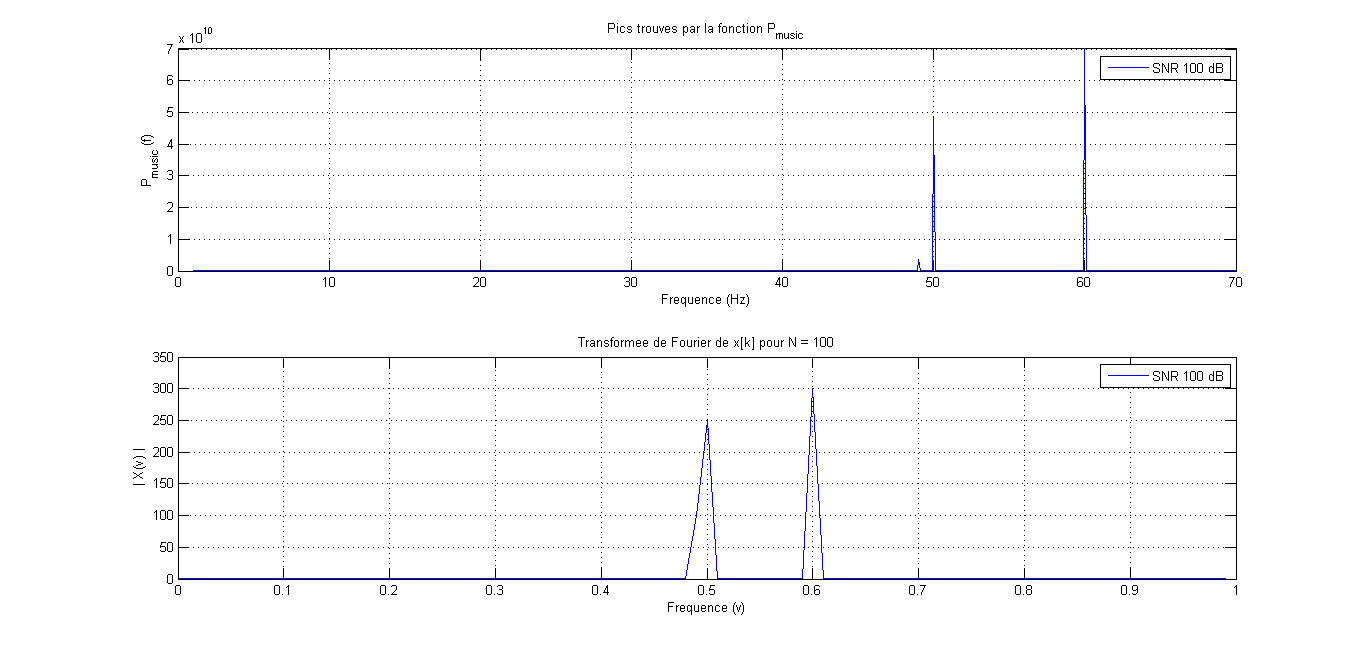
\includegraphics[scale=\rapportFigureMoyenne ]{images/snr100}
        \caption{ \(SNR_{dB} = 100 dB\)}
        \label{fig:snr100}
    \end{subfigure}
    
    \caption{Resultats obtenus pour différentes valeurs du SNR}
%
\end{figure}

\FloatBarrier


Finalement, un dernier exemple, répresenté par la figure \ref{fig:snr500}, qui illustre le cas où le bruit interfère de façon très faible sur le signal (comparer avec le premier cas, en regardant les figures \ref{fig:wave500} et \ref{fig:wave0001}). Dans ce cas là, la puissance du signal est \(10^{50}\) plus forte que celle du bruit et on obtient , comme espéré, les trois pics bien définis pour la fonction P\textsuperscript{music}. On note notamment que les deux fréquences très proches ont pu être bien distingué. Cependant, le résultat relatif à la \textit{fft} n'a pas montré d'avancés significatives: les fréquences \(f_1\) et \(f_2\) n'ont pas pu être différencié quand même.

\FloatBarrier


\begin{figure}[h]
%
    \centering
    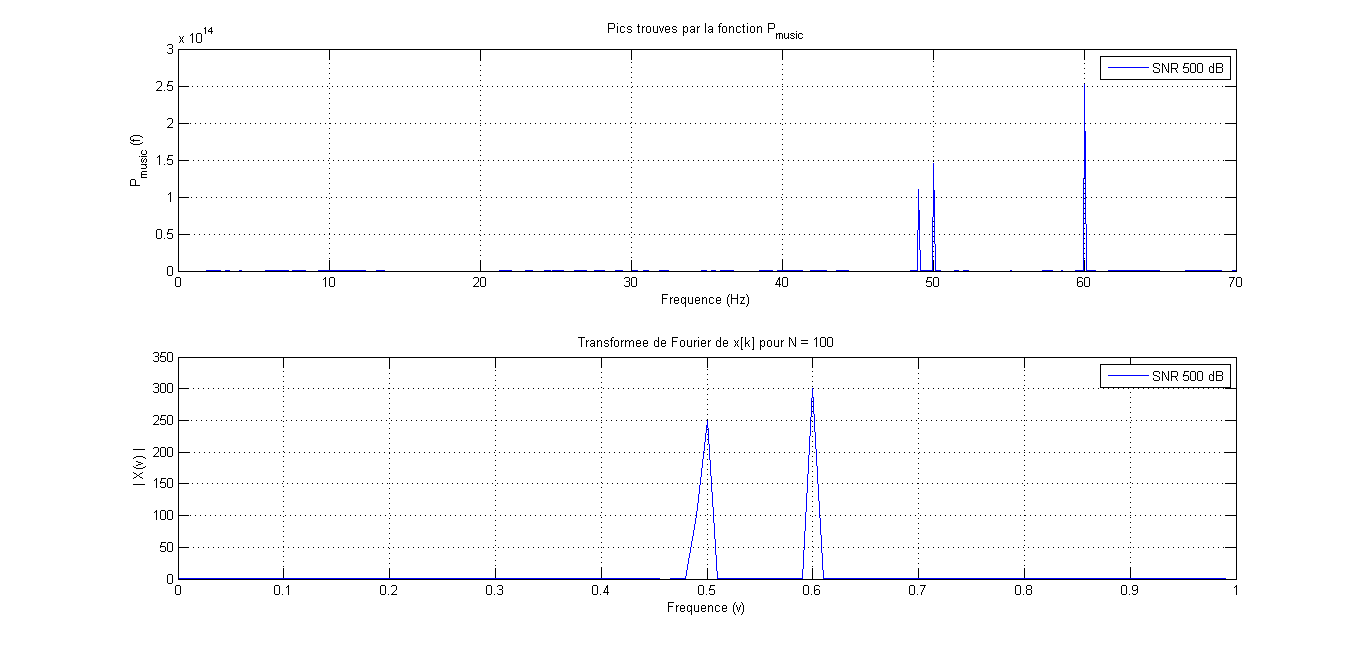
\includegraphics[scale=\rapportFigure ]{images/snr500}
    \caption{Resultats obtenus pour \(SNR_{dB} = 500 dB\)}
    \label{fig:snr500}
\end{figure}
%

\begin{figure}[h]
%
    \centering
    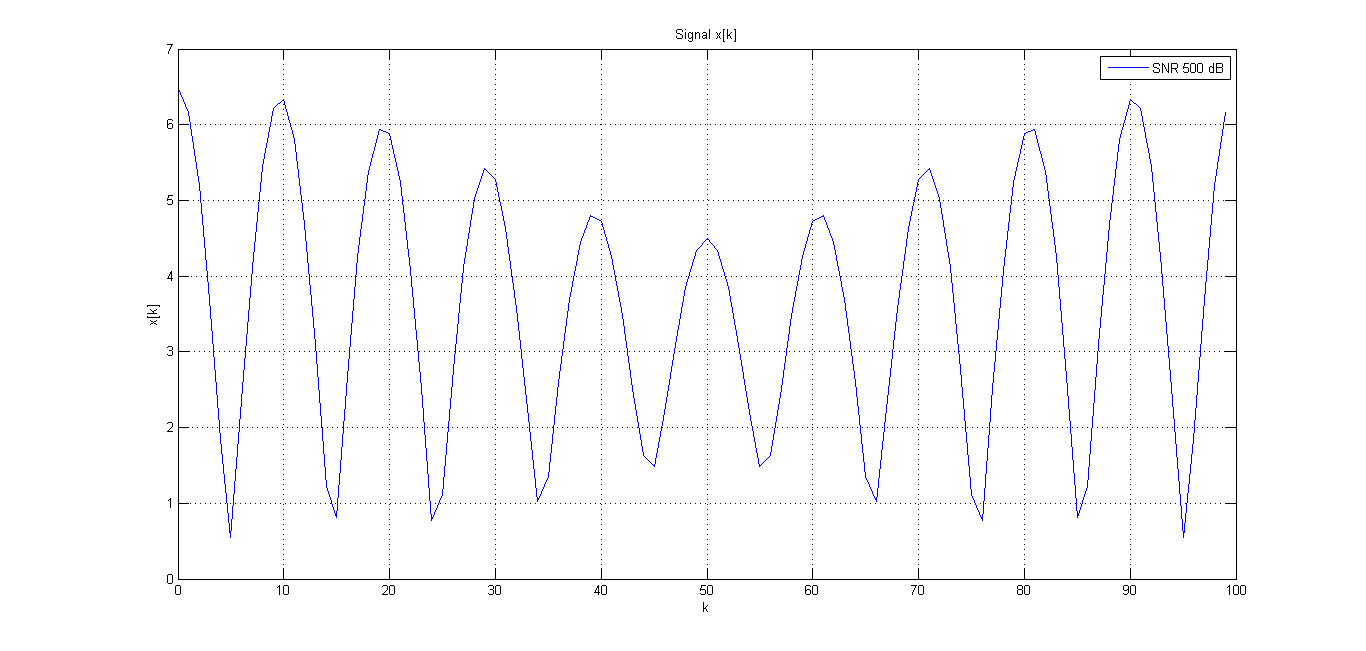
\includegraphics[scale=\rapportFigure ]{images/wave500}
    \caption{Signal pour \(SNR_{dB} = 500 dB\)}
    \label{fig:wave500}
\end{figure}
%

\newpage

\section{Algorithme ESPRIT}

ESPRIT (Estimation of Signal Parameters via Rotational Invariance Techniques) est une méthode de localisation de sources mais qui ne s'applique que dans le cas particulier d'un réseau de capteurs constitués de deux sous-antennes identiques translatés l'une par rapport à l'autre. Elle a été implémenté afin de gagner en temps de calcul par rapport aux algorithmes plus conventionels comme MUSIC. Son succès repose également sur sa simplicité et ses bonnes performances.

\vspace*{10pt}

On considère toujours le même le processus \(x[n] = s[n] + w[n]\) où \(w[n]\) est un bruit blanc \(w[n]\) de variance \(p_w\) et s[n] est défini comme pour l'équation \ref{eq:x}.

Supposons que les antennes soient disposées comme ci-dessous:

\begin{figure}[h]
\centering
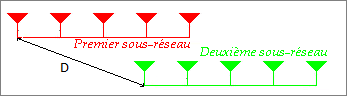
\includegraphics[scale=.8]{images/ReseauEsprit}
\caption{Disposition des antennes.}
\end{figure}

On a un déphasage temporel de \( \frac{D sin(\phi) }{c}  \) entre les 2 capteurs qui se correspondent où c est la célérité de la lumière et \(\phi\) l'angle d'incidence du signal. Soit N le nombre de capteurs d'un réseau. 


Ainsi on peut écrire que 

\begin{equation}
S_2 = S_1 \Omega
\end{equation}

\vspace*{20pt}

si \[ S_1 = \begin{bmatrix}
        \boldsymbol{e}_{N-1}(f_1) & \cdots & \boldsymbol{e}_{N-1}(f_P)
    \end{bmatrix} \] avec \( \boldsymbol{e}_{N-1}(f_k) \) définie comme en \ref{eq:em}
    


    
\vspace*{20pt}

et \[ \Omega = \begin{bmatrix}
         \exp(2\pi j f_1 \frac{D sin(\phi_1) }{c}) & & \text{\huge0}\\
         &  \ddots \\
         \text{\huge0} & & \exp(2\pi j f_p \frac{D sin(\phi_P) }{c})\\

         \end{bmatrix} \]
        
\vspace*{20pt}
         
La matrice d'autocorrélation s'écrit alors 

\begin{equation}
R_{xx} = R_{ss} + R_w =\sum_{k=1}^{P}A_k^2 \begin{bmatrix} \boldsymbol{e}_{N-1}(f_k) \\ \boldsymbol{e}_{N-1}(f_k) \exp(2\pi j f_k \frac{D sin(\phi_k) }{c}) \end{bmatrix} \begin{bmatrix} \boldsymbol{e}_{N-1}(f_k) \\ \boldsymbol{e}_{N-1}(f_k) \exp(2\pi j f_k \frac{D sin(\phi_k) }{c}) \end{bmatrix}^H + p_w\boldsymbol{I}
\end{equation}

\vspace*{20pt}

ou encore

\begin{equation}
R_{xx} = \begin{bmatrix} S_1 \\ S_1 \Omega \end{bmatrix} 
\begin{bmatrix} A_1^2 & & \text{0}\\ &  \ddots \\ \text{0} & & A_P^2 \\ \end{bmatrix}
\begin{bmatrix}   S_1 \\ S_1 \Omega \end{bmatrix}^H  + p_w\boldsymbol{I}
\end{equation}

Celle-ci possède 2N valeurs propres et les P plus grandes correspondent à l'espace signal.
Les vecteurs propres associés notés \( u_1, ..., u_P \) engendrent l'espace signal tout comme les colonnes de la matrice des vecteurs sources \( \begin{bmatrix} S_1 \\ S_1 \Omega \end{bmatrix} \).
Ainsi il existe une matrice T inversible telle que:

\begin{equation}
U = [u_1 \cdots u_P] = \begin{bmatrix} U_1 \\ U_2 \end{bmatrix} = \begin{bmatrix} S_1 \\ S_1 \Omega \end{bmatrix} T = \begin{bmatrix} S_1 T \\ S_1 \Omega T \end{bmatrix}
\end{equation}

\vspace*{20pt}

Ainsi \( S_1 = U_1 T^{-1}\) et \( U_2 = S_1 \Omega T \) ce qui donne :

\begin{equation}
U_2 = U_1 T^{-1} \Omega T = U_1 \Psi
\end{equation}

\( \Psi \) possède les mêmes valeurs propres que \( \Omega \). Donc la connaissance de cette matrice permet d'obtenir les informations sur le signal. Pour obtenir une estimation de \(\Psi\), on utilise communément le critère des moindres carrés qui donne:

\begin{equation}
\Psi = (U_1 U_1^H)^{-1} U_1^H U_2
\end{equation}



%http://telice.univ-lille1.fr/fileadmin/general/theses/PaulStefanut_2010_2.pdf
%http://tel.archives-ouvertes.fr/docs/00/44/74/88/PDF/These_Carine_EK.pdf
%http://perso.telecom-paristech.fr/~rioul/liesse/2012liesse4/YG-slides.pdf
%A_1 \exp(j \theta _1)) & \cdots &  A_P \exp(j \theta _P)) \\
%        \vdots & \ddots &  \vdots\\
%        A_1 \exp(j(2\pi f_0 (N-1) T + \theta _1)) &  \cdots & A_P \exp(j(2\pi f_0 (N-1) T + \theta _P)) %\\
\newpage

%\bibliographystyle{plain}
%\bibliography{bibliographie}

\section {Références}

\begin{itemize}
\item 
Institute for Dynamics Systems and Control. \textit{White noise and power spectral density}.\\
\url{http://www.idsc.ethz.ch/Courses/signals_and_systems/ArchiveFall10/lectureNotes8.pdf}

\item S. Lawrence Marple Jr. \textit{Digital Spectral Analysis with Applications}. Prentice-Hall Inc, 1988

\item Bernard Picinbono. \textit{Signaux aléatoires - Tome 2 Fonctions aléatoires et modèles avec problèmes résolus}. Dunod Université, 1993

\item \textit{Les méthodes à haute résolution}. HERMES, 1998

\item Yves Grenier. \textit{Méthodes haute-résolution en analyse spectrale et localisation}. \\
\url{http://perso.telecom-paristech.fr/~rioul/liesse/2012liesse4/YG-slides.pdf}

\end{itemize}


\end{document}
